\hypertarget{tiempo-hasta-el-cierre}{%
\section{Tiempo hasta el cierre}\label{tiempo-hasta-el-cierre}}

Pregunta: ¿Cuánto tiempo pasa entre la creación y el cierre de una
operación, como una incidencia, una revisión o un ticket de soporte?

\hypertarget{descripciuxf3n}{%
\subsection{Descripción}\label{descripciuxf3n}}

El tiempo hasta el cierre es la cantidad total de tiempo que transcurre
entre la creación y el cierre de una operación como una incidencia, una
revisión o un ticket de soporte. La operación debe tener un estado
abierto y cerrado, como suele ser el caso en los procesos de revisión de
código, foros de preguntas y respuestas y sistemas de emisión de
tickets.

Métrica relacionada:
\href{https://chaoss.community/metric-issue-resolution-duration/}{Duración
de la resolución de la incidencia}

\hypertarget{objetivos}{%
\subsection{Objetivos}\label{objetivos}}

\begin{enumerate}
\tightlist
\item
  Determinar en qué medida lo receptiva que sea una comunidad puede
  ayudar a que los esfuerzos sean inclusivos, atraigan y retengan
  contribuyentes nuevos y existentes.
\item
  Identificar las características de las operaciones que afectan a que
  una operación se cierre de forma rápida o lenta (por ejemplo,
  encontrar las mejores prácticas, áreas de mejora, evaluar la
  eficiencia).
\item
  Identificar sesgos para respuestas oportunas a diferentes miembros de
  la comunidad.
\item
  Detectar un cambio en la actividad de la comunidad (por ejemplo, para
  indicar un posible agotamiento del mantenedor, reducción en la
  diversidad de las contribuciones)
\end{enumerate}

\hypertarget{implementaciuxf3n}{%
\subsection{Implementación}\label{implementaciuxf3n}}

\hypertarget{filtros}{%
\subsubsection{Filtros}\label{filtros}}

\begin{itemize}
\tightlist
\item
  Creador de la operación (p. ej., nuevo contribuyente vs. mantenedor)
\item
  Primero cerrado, final cerrado
\item
  etiquetas de incidencias (p. ej., error vs. nueva característica)
\end{itemize}

\hypertarget{visualizaciones}{%
\subsubsection{Visualizaciones}\label{visualizaciones}}

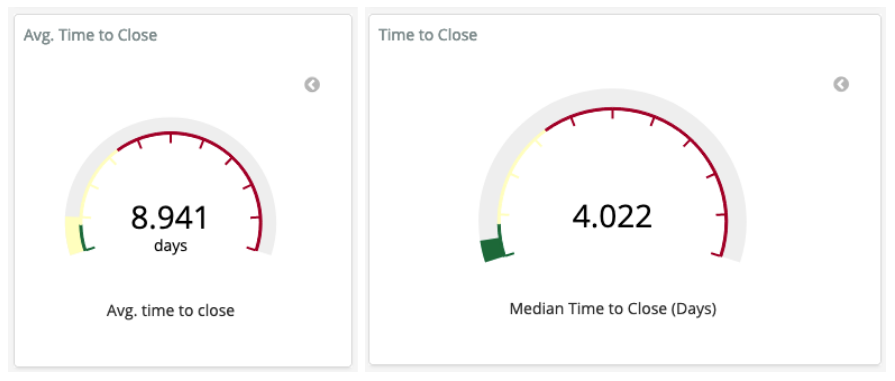
\includegraphics{images/time-to-close_1.png}

\hypertarget{herramientas-que-proporcionan-la-muxe9trica}{%
\subsubsection{Herramientas que proporcionan la
métrica}\label{herramientas-que-proporcionan-la-muxe9trica}}

Implementación de Augur:

\begin{itemize}
\tightlist
\item
  \href{http://augur.osshealth.io/api_docs/\#api-Evolution-Closed_Issue_Resolution_Duration(Repo)}{Duración
  del cierre de la incidencia}
\item
  \href{http://augur.osshealth.io/api_docs/\#api-Evolution-issue-duration-repo}{Duración
  de la incidencia}
\item
  \href{http://augur.osshealth.io/api_docs/\#api-Evolution-Issue_Response_Time(Repo)}{Tiempo
  de respuesta a la incidencia}
\end{itemize}

Implementación de GrimoireLab:

\begin{itemize}
\tightlist
\item
  \href{https://chaoss.github.io/grimoirelab-sigils/panels/github-pullrequests-efficiency/}{Eficiencia
  de las solicitudes de extracción}
\item
  \href{https://chaoss.github.io/grimoirelab-sigils/panels/github-issues-efficiency/}{Eficiencia
  de las incidencias}
\item
  \href{https://chaoss.github.io/grimoirelab-sigils/panels/efficiency-timing-overview/}{Efficiency:TimingOverview}
\end{itemize}

\hypertarget{estrategias-de-recopilaciuxf3n-de-datos}{%
\subsubsection{Estrategias de recopilación de
datos}\label{estrategias-de-recopilaciuxf3n-de-datos}}

El tiempo para cerrar la métrica puede ser contextual según la actividad
y los objetivos del proyecto. Por ejemplo, el tiempo que se tarda en
cerrar un informe de errores puede proporcionar información diferente
que el tiempo que se tarda en cerrar una nueva solicitud de función. Las
estrategias de recopilación de datos deben abordar diferentes objetivos
del proyecto. Otras variables que pueden influir en estos procesos son:

\begin{itemize}
\tightlist
\item
  Sistemas de seguimiento de incidencias: el tipo de incidencia, como
  informe de error, plan (nomenclatura de OpenStack), historial del
  usuario, solicitud de función, épica y otros, puede influir en el
  tiempo que tarda en cerrarse este evento. Otras variables, como la
  prioridad o la gravedad, pueden ayudar a anticipar la rapidez con la
  que se cerrará este evento.
\item
  Procesos de revisión de código: esto depende de la infraestructura de
  revisión de código, como Gerrit, GitHub o listas de correo (como en el
  Kernel de Linux) y puede diferir dependiendo de lo complicado que sea
  el proceso. Por ejemplo, los desarrolladores recién llegados o
  avanzados y experimentados procederán de diferentes maneras y
  requerirán de más o menos tiempo.
\item
  Foro de preguntas y respuestas: depende de la calidad de la respuesta
  y de la opinión de la persona que hace la pregunta. Se marca una
  respuesta válida y el proceso se cierra una vez que la persona que
  pregunta ha encontrado con éxito una respuesta correcta a su pregunta.
\end{itemize}

\hypertarget{referencias}{%
\subsection{Referencias}\label{referencias}}

\begin{itemize}
\tightlist
\item
  «Practice P.12: Respond to all submissions» de «Appendix to: Managing
  Episodic Volunteers in Free/Libre/Open Source Software Communities» de
  Ann Barcomb, Klaas-Jan Stol, Brian Fitzgerald y Dirk Riehle:
  \url{https://opus4.kobv.de/opus4-fau/frontdoor/index/index/docId/13519}
\end{itemize}
